% !TeX root = ../main.tex
% Add the above to each chapter to make compiling the PDF easier in some editors.
%------------------------------------------------------------------------
\chapter{Tuning Linear Programming Solvers for Query Optimization}\label{chapter:linearprogramming}

%------------------------------------------------------------------------
%------------------------------------------------------------------------
\section{Proposal or Implementation}
Our contribution consists in conducting experiments on small packing LP problems that are generated from
real-life queries as mentioned in Section \ref{section:cardinality-estimate} as well as randomly generated
LPs with varying sizes. We use different LP solvers, and different update methods to solve these LPs.
We then proceed to compare results based on time and memory performance. We also build an analysis of our datasets' properties.
Finally, we aim to give a recommendation on how to build the best performing LP solver based on the
particularities of the LP problems.

%------------------------------------------------------------------------
\subsection{Implementation hierarchy}
The final code repository contains 3 different solvers as shown in the
UML graph \ref{fig:hierarchy}
and a \verb|compareSolvers.cpp|, in which we can conduct our benchmarks.
\begin{figure}[htpb]
    \centering
    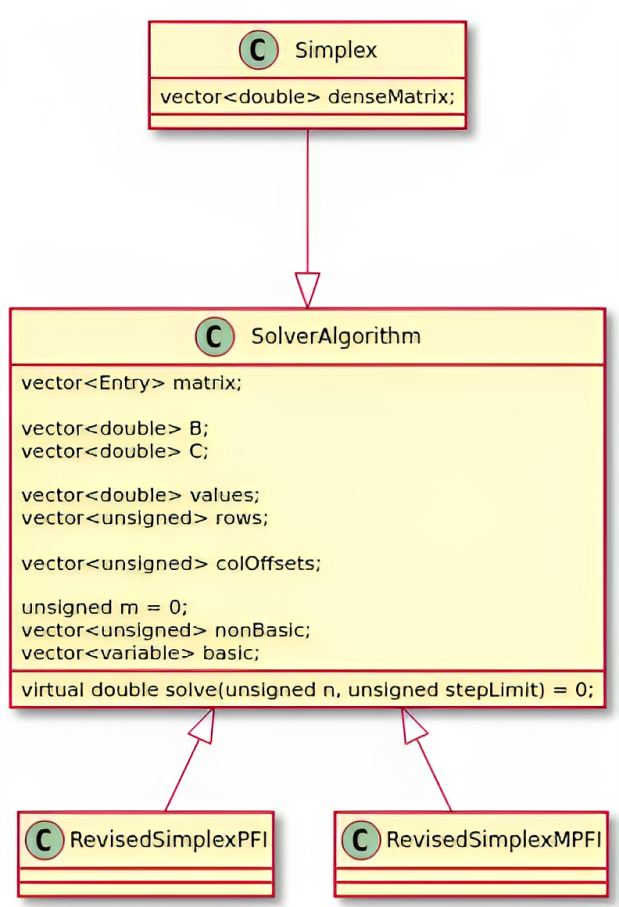
\includegraphics[height=0.6\textheight]{figures/UML.png}
    \caption{An UML Graph explaining the hierarchy of the implementation}
    \label{fig:hierarchy}
\end{figure}

%------------------------------------------------------------------------
\subsection{Tableau simplex solver}
This solver is the simplest of the three solvers, it follows the steps of the standard simplex 
algorithm in its tabular form. It uses dense matrices and vectors. Although the
doPivotting() is costly, the simplicity of this algorithm makes it suitable for 
smaller problems.
\begin{algorithm}
    \caption{Tableau Simplex Algorithm}
    \begin{algorithmic}[1]
        \State \textbf{Input:} Packing LP maximisation problem in computational form
        \State \textbf{Output:} Optimal value $z$

        \State \textbf{Step 1:} Pricing: Find pivot column, or entering variable using Bland's rule
        \State \hspace{\algorithmicindent} $enteringVars \gets \text{findPivotColumnCandidates}()$
        \State \hspace{\algorithmicindent} \textbf{if} no entering variable found \textbf{then}
        \State \hspace{\algorithmicindent} \hspace{\algorithmicindent} \text{print} "Optimal value reached."
        \State \hspace{\algorithmicindent} \hspace{\algorithmicindent} \Return $z$
        \State \hspace{\algorithmicindent} \textbf{end if}
        \State \hspace{\algorithmicindent} $pivotColumn \gets enteringVars[0]$

        \State \textbf{Step 2:} Find pivot row, or leaving variable using the ratio test
        \State \hspace{\algorithmicindent} $pivotRow \gets \text{findPivotRow}(pivotColumn)$
        \State \hspace{\algorithmicindent} \textbf{if} no leaving variable \textbf{then}
        \State \hspace{\algorithmicindent} \hspace{\algorithmicindent} \text{print} "The given LP is unbounded."
        \State \hspace{\algorithmicindent} \hspace{\algorithmicindent} \Return $\infty$
        \State \hspace{\algorithmicindent} \textbf{end if}

        \State \textbf{Step 3:} Update the tableau using pivotting and update the objective function value
        \State \hspace{\algorithmicindent} $\text{doPivotting}(pivotRow, pivotColumn, z)$

        \State \textbf{Goto Step 1}
    \end{algorithmic}
\end{algorithm}
%------------------------------------------------------------------------
\subsection{Data structures}

\subsubsection{Dense Matrix}
Given a matrix \( A \) of dimensions \( m \times n \), the density \( D \) of
the matrix is defined as:
\[
    D(A) = \frac{\text{Number of non-zero elements in } A}{m \times n}
\]
$D$ is a measure between 0 and 1, where 0 indicates a
matrix with all zero elements (completely sparse)
and 1 indicates a matrix with all non-zero elements (completely dense).
Sparsity of a matrix is a feature that can be exploited to
enhance memory complexity of our implementation, as we will discuss next.

\subsubsection{Sparse Matrix}\label{subsubsection:sparse-matrix}
In our dataset, we deal with sparse matrices.
We use the \gls{ccr} format to store sparse matrices in C++. They are represented using this
structure.

\begin{verbatim}
      struct CCRMatrix {
          float *values;  // Non-zero values in the matrix
          int *rowIdx;  // Row indices corresponding to the non-zero values
          int *colPtr;  // Points to the index in `values` where each column starts
      };
\end{verbatim}

For example, consider the matrix \( A \):
\[
    A =
    \begin{bmatrix}
        5 & 0 & 0 \\
        0 & 8 & 0 \\
        0 & 0 & 3 \\
        0 & 6 & 0 \\
    \end{bmatrix}
\]

In \gls{ccr} format, the matrix is represented using three arrays:
\texttt{values}, \texttt{row\_indices}, and \texttt{column\_pointers}.

\begin{align*}
    \texttt{values}           & = [5, 8, 6, 3] \\
    \texttt{row\_indices}     & = [0, 1, 3, 2] \\
    \texttt{column\_pointers} & = [0, 1, 3, 4] \\
\end{align*}
\subsubsection{Comparison of memory complexity}
Storing a dense matrix variable \( A \) of dimensions \( m \times n \) in C++, we have two alternatives.
\begin{itemize}
    \item using an array of arrays (two-dimensional array) or \texttt{vector<vector<double>>}. This array would contain
          $m$ arrays, representing the rows, each contains $n$ doubles, representing the matrix entries in each row.
    \item using a one-dimensional array with rows stacked next to each other,
          \texttt{vector<vector<double>>}. This array contains $m \times n$ entries.
          With the $a_{row,col}$ entry located at \texttt{A[row * (m + n) + col]}
\end{itemize}
Note that even
though there is a difference between  \texttt{array}, \texttt{vector} and \texttt{list}, we
choose \texttt{std::vector}, or dynamoic array, in all our implementation, because it suits our purpouses.
We also opt for 1D array as opposed to 2D array for better memory complexity and speed.
We explain this choice:
The 2D array typically requires slightly more memory than its 1D counterpart.
This increased memory usage is attributed to the pointers in the 2D array that point to
the set of allocated 1D arrays. While this difference might seem negligible for large arrays,
it becomes relatively significant for smaller arrays. In terms of speed, the 1D array often outperforms
the 2D array due to its contiguous memory allocation, which reduces cache misses.
However, the 2D dynamic array loses cache locality and consumes more memory because of its non-contiguous
memory allocation. While the 2D dynamic array introduces an
extra level of indirection, the 1D array has its own overhead stemming from index calculations.

\begin{figure}[h]
    \centering
    \caption{Memory Layout of a 1D Dynamic Array}
    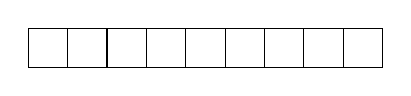
\begin{tikzpicture}[scale=0.5, every node/.style={scale=0.5}]
        \foreach \x in {0,...,8} {
                \draw (\x,0) rectangle ++(1,1);
            }
    \end{tikzpicture}
\end{figure}

\begin{figure}[h]
    \centering
    \caption{Memory Layout of a 2D Dynamic Array}
    \begin{tikzpicture}[scale=0.5, every node/.style={scale=0.5}]
        \foreach \x in {0,...,2} {
                \draw (\x,2) rectangle ++(1,1);
            }
        \foreach \x in {0,...,2} {
                \foreach \y in {0,...,2} {
                        \draw (\x*4+\y,-\x) rectangle ++(1,1);
                    }
            }
        \draw[->] (0.5,2) -- (0.5,1);
        \draw[->] (1.5,2) -- (1.5,1.25) -- (4.5,1.25) -- (4.5,0);
        \draw[->] (2.5,2) -- (2.5,1.5) -- (8.5,1.5) -- (8.5,-1);
    \end{tikzpicture}
\end{figure}


%------------------------------------------------------------------------
\subsection{Revised Simplex Solver}


%------------------------------------------------------------------------
\subsection{Stability}
Mention zero tolerances: A zero tolerance epsilon2 saefguards against divisions
by extremely small numbers, which tend to produce the most dangerous rounding errors, and
may even lead to degeneracy. diagonal entry in eta matrix should be fairly far from
otherwise (in our experiment) degeneracy.

%------------------------------------------------------------------------

%------------------------------------------------------------------------
\section{Experiments and Results}
All the following results have been obtained on a system with the following settings:
\begin{itemize}
    \item OS: Ubuntu 22.04.1 LTS x86\_64
    \item Host: 82A2 Yoga Slim 7 14ARE05

    \item CPU: AMD Ryzen 7 4800U with Radeon Graphics (16) @ 1.800GHz
    \item GPU: AMD ATI 03:00.0 Renoir
    \item Memory: 10409MiB / 15363MiB
\end{itemize}

Presolve techniques are not used, the solvers assume an input of the form explained
in the UML graph \ref{fig:hierarchy} and in the format input as described in the following section.

The computed optimal solutions have been validated using the scipy python library.

%------------------------------------------------------------------------
\subsection{Query datasets}
The input files \texttt{TPCH}, \texttt{TPCDS}, and \texttt{JOB} contain packing
\gls{lp} problems. We have already established the mathematical derivation of how
these query-related packing
\gls{lp} problems are generated in \ref{subsection:cardinality-estimate}.

The \texttt{lp.txt} file is structured for machine readability.
In this format, each line represents a single \gls{lp}. The line starts with
the number of rules in that problem. For each rule, the number of entries in
the coefficient matrix is specified first, followed by pairs of values:
the column number and the coefficient. This is convenient to parse the entries
and then populate our sparse matrix representation quite efficiently.

\begin{lstlisting}
lp:
8 2 0 0.0540277 2 0.0540277 ...
\end{lstlisting} \label{format_input}

\begin{table}[!htb]
    \centering
    \caption{Benchmarks and workloads.}
    \begin{tabular}{|l|l|}
        \hline
        Benchmark                                & Number of Queries \\
        \hline
        JOB \parencite{10.14778/2850583.2850594} & 2230              \\
        TPC-H \parencite{tpch}                   & 16                \\
        TPC-DS \parencite{tpcds2022}             & 148               \\
        \hline
    \end{tabular}
\end{table}

\subsubsection{The JOB dataset results}
In the table \ref{table_job_stats} are some important statistical finds following our
experiments with the JOB dataset.
This is the largest dataset of all three query datasets. It contains duplicated queries so we
perform a removal of the duplicated LPs before. We collect the data and perform plotting and data summary
using R scripts.

\begin{figure}[!htb]
    \centering
    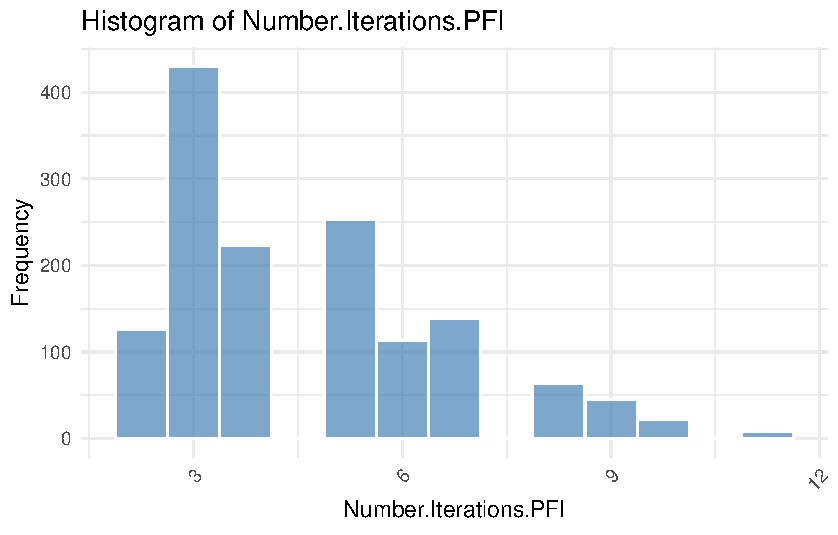
\includegraphics[width=\textwidth]{figures/histo_iter_pfi.pdf}
    \caption{Boxplot for number of iterations for PFI for JOB dataset}
    \label{fig:num_iter_boxplot_pfi_job}
\end{figure}

\begin{figure}[!htb]
    \centering
    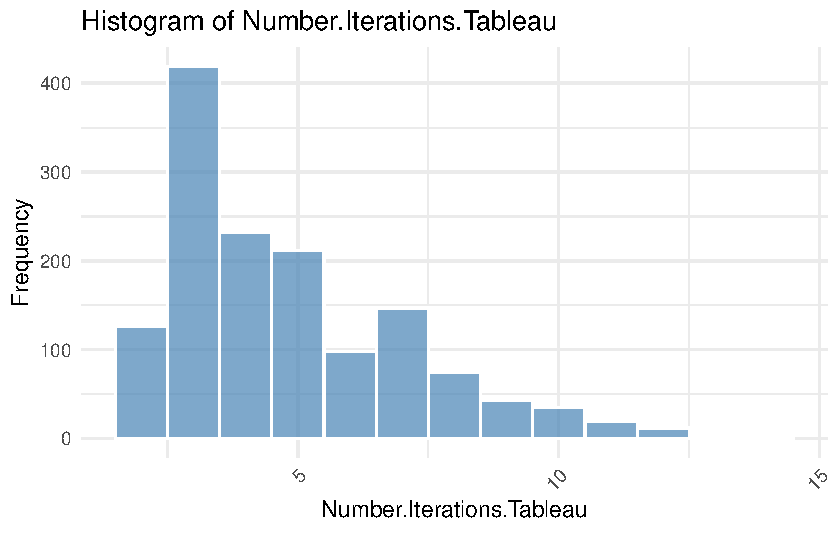
\includegraphics[width=\textwidth]{figures/histogram_iter_tableau.pdf}
    \caption{Boxplot for number of iterations for Tableau for JOB dataset}
    \label{fig:num_iter_boxplot_tableau_job}
\end{figure}


\begin{figure}[!htb]
    \centering
    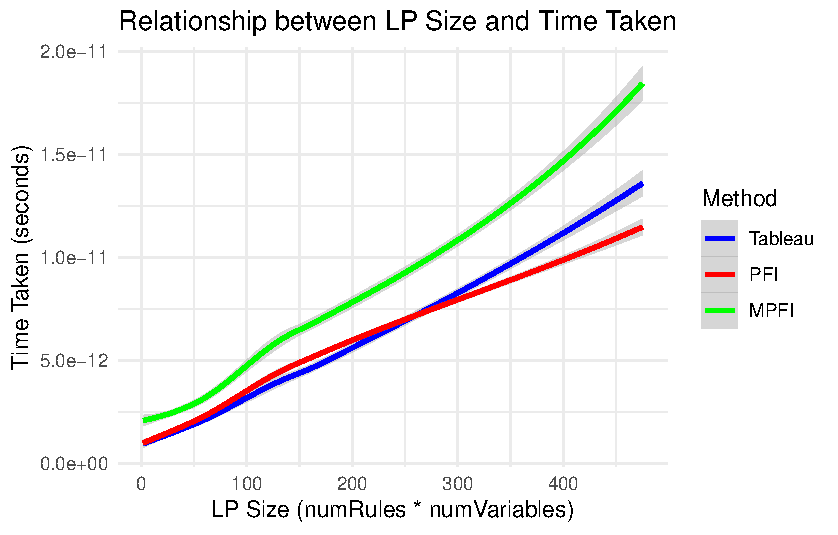
\includegraphics[width=\textwidth]{figures/lp_size_vs_time_job.pdf}
    \caption{Relation between LP size and time for the 3 simplex solvers for JOB dataset.}
    \label{fig:lp_size_vs_time_job}
\end{figure}

\begin{table}[!htb]
    \centering
    \caption{Statistics about JOB dataset}
    \begin{tabular}{lrrrr}
        \toprule
        Variable                  & Min    & Median  & Mean    & Max     \\
        \midrule
        LP size                   & 2.00   & 54.00   & 94.56   & 475.00  \\
        Number of Rules           & 1.000  & 6.000   & 7.037   & 19.000  \\
        Number of Variables       & 1.00   & 3.00    & 3.07    & 6.00    \\
        Constraint Matrix Density & 0.3684 & 0.6667  & 0.6703  & 1.0000  \\
        Solution Time Scipy       & 650    & 931     & 959     & 1802    \\
        Solution Time Scipy       & 97.04  & 184.06  & 190.66  & 415.56  \\
        Solution Time Tableau     & 2.00   & 4.00    & 12.15   & 4274.00 \\
        Solution Time PFI         & 2.000  & 6.000   & 8.316   & 65.000  \\
        Solution Time MPFI        & 1.000  & 4.000   & 5.517   & 68.000  \\
        Number Iterations Tableau & 2.000  & 4.000   & 4.829   & 14.000  \\
        Number Iterations PFI     & 2.000  & 4.000   & 4.621   & 11.000  \\
        Number Iterations MPFI    & 2.000  & 4.000   & 4.671   & 13.000  \\
        Optimal Value             & 0.3188 & 20.6702 & 21.8575 & 42.1804 \\
        \bottomrule
    \end{tabular}
\end{table} \label{table_job_stats}

This is our results:
\begin{table}[!htb]
    \centering
    \caption{Number of LPs or Queries Solved by Hour for the JOB dataset}
    \begin{tabular}{l|r}
        \toprule
        Method                     & Number of LPs/Queries \\
        \midrule
        Revised Simplex MPFU Umbra & 906,607,929           \\
        Tableau Simplex            & 1,400,923,787         \\
        Revised Simplex PFI        & 1,287,140,216         \\
        Scipy (method highs)       & 4,069,108             \\
        Cplex                      & 17,849,851            \\
        \bottomrule
    \end{tabular}
\end{table}


\begin{figure}[p]
    \begin{adjustbox}{width=\paperwidth,center}
        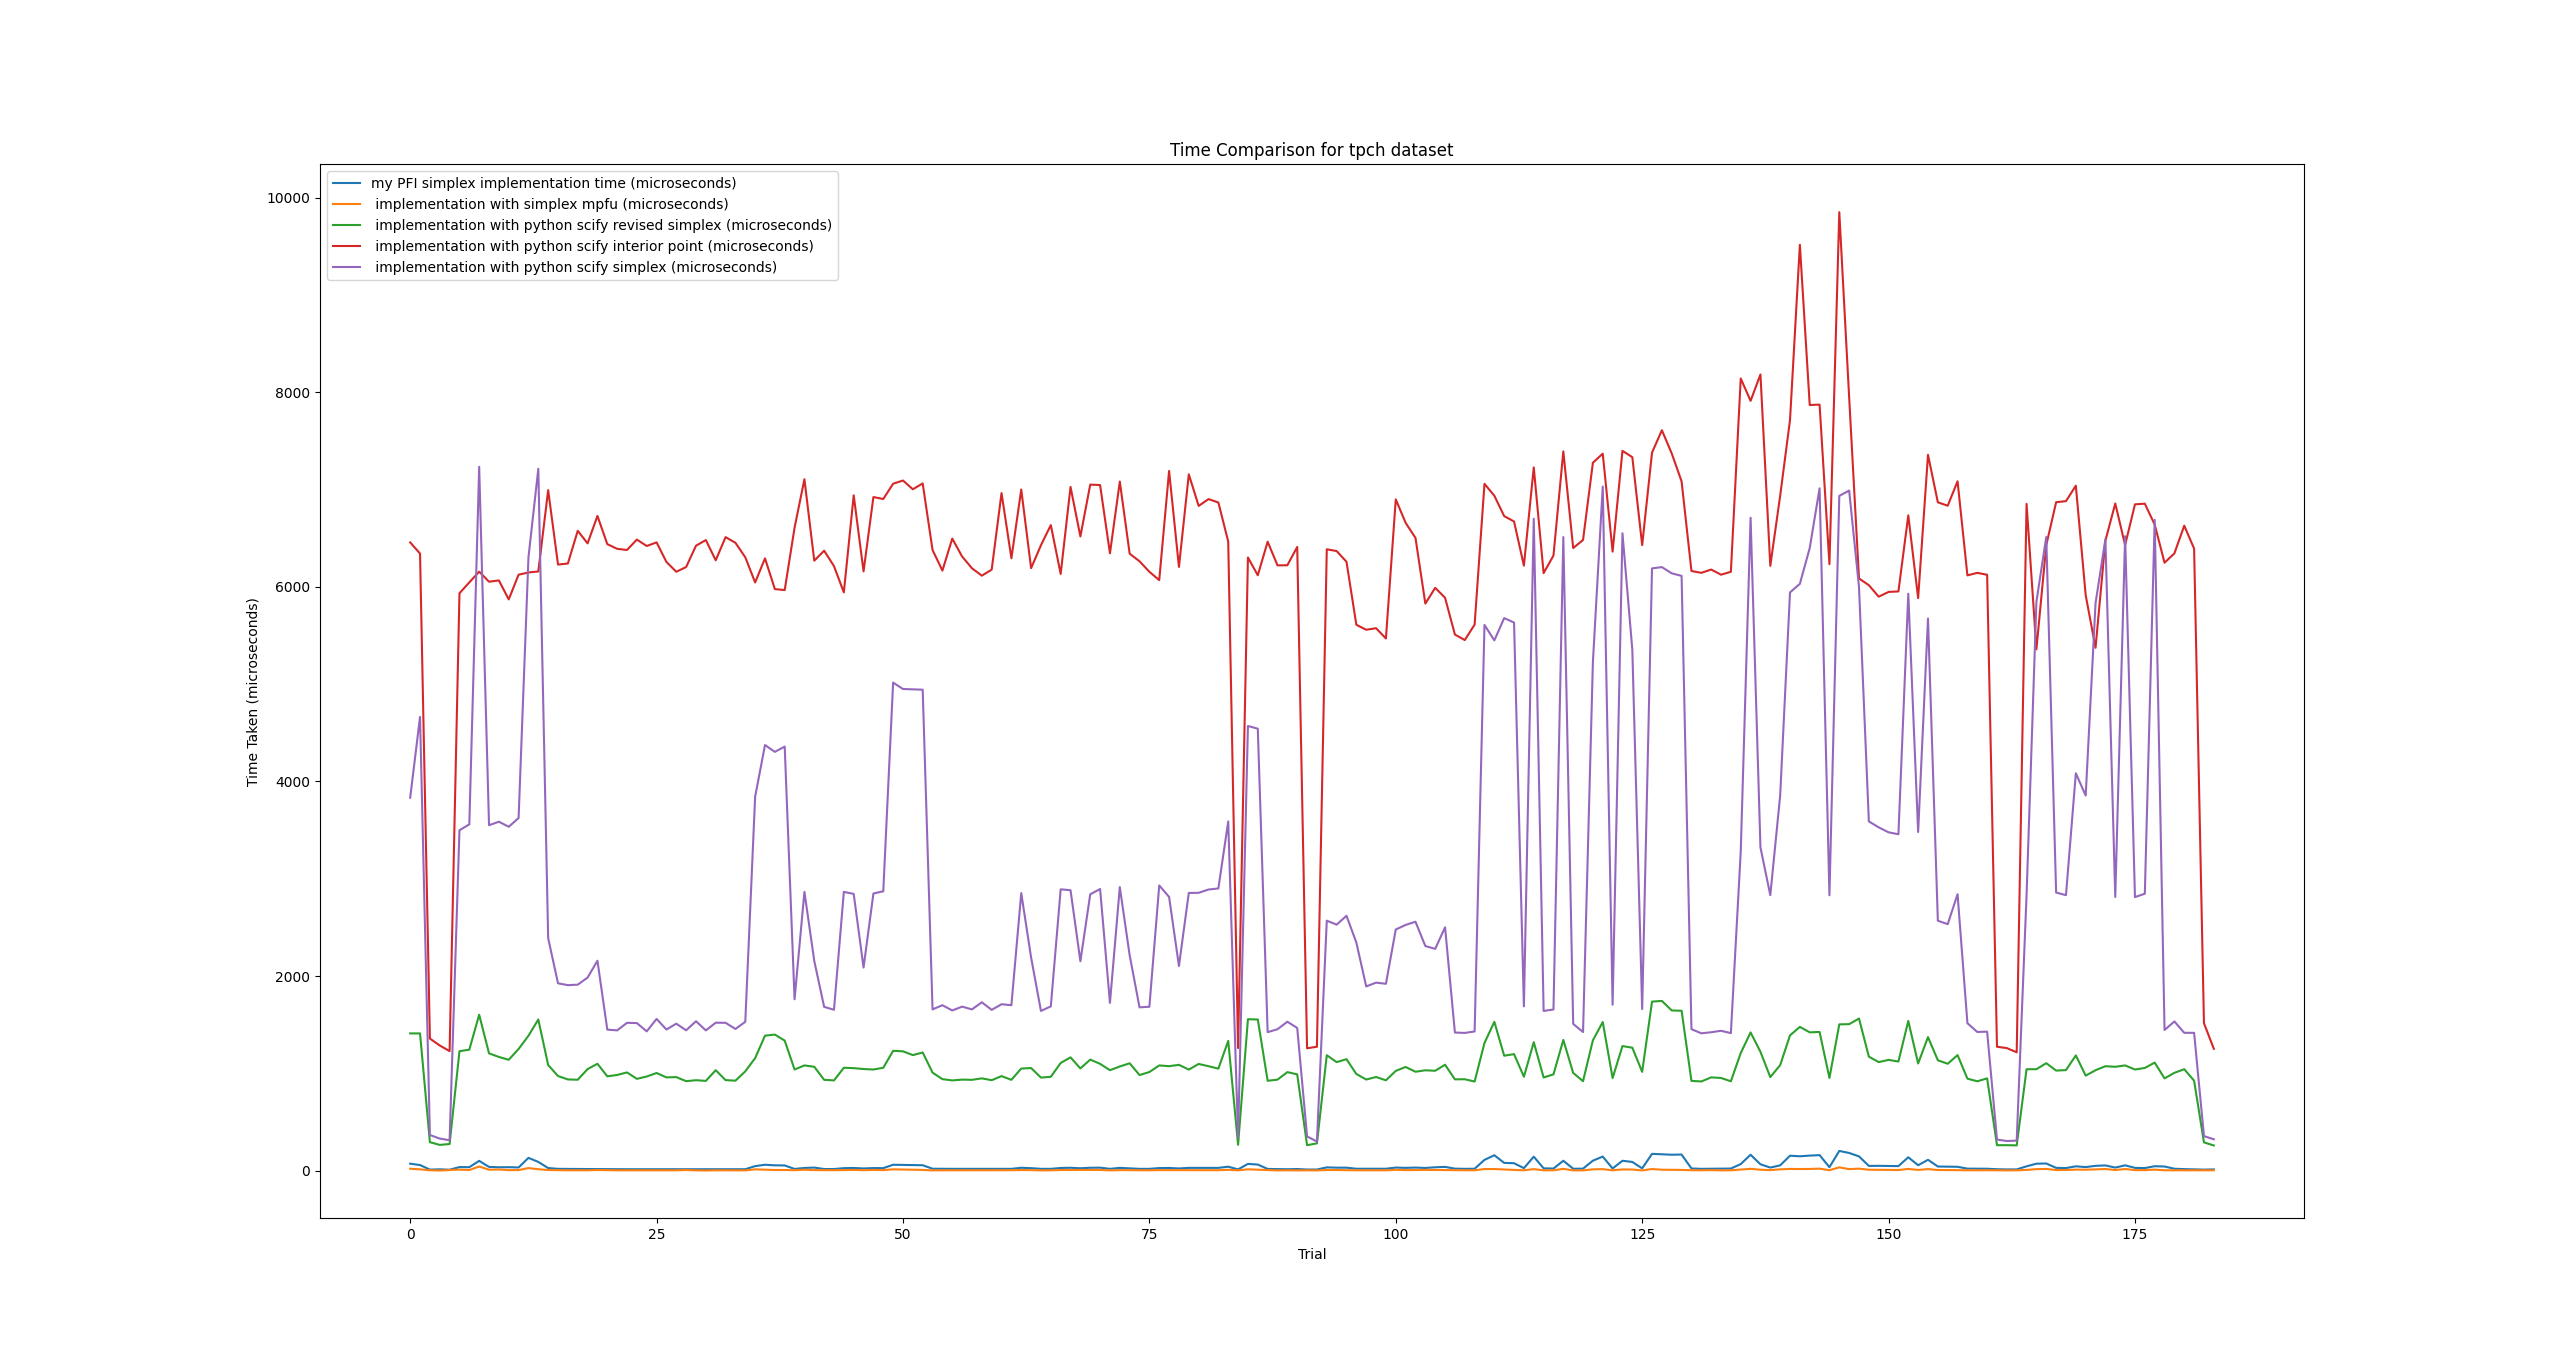
\includegraphics[width=\paperwidth]{figures/all_scify_mpfi_pfi.png}
    \end{adjustbox}
    \caption{A graph comparing the time performance of two of
        our solvers with scipy solver solving the tpch dataset}
    \label{fig:all_time_tpch}
\end{figure}




\subsubsection{TPC-DS results}

%------------------------------------------------------------------------
\subsection{Results on randomly generated LPs}
We also test our solvers alongside Cplex, on packing LPs generated randomly. We want to 
explore those results to investigate how these solvers scale, and if the speedup
they provide is still substantial at larger LPs.


\begin{figure}[!htb]
    \centering
    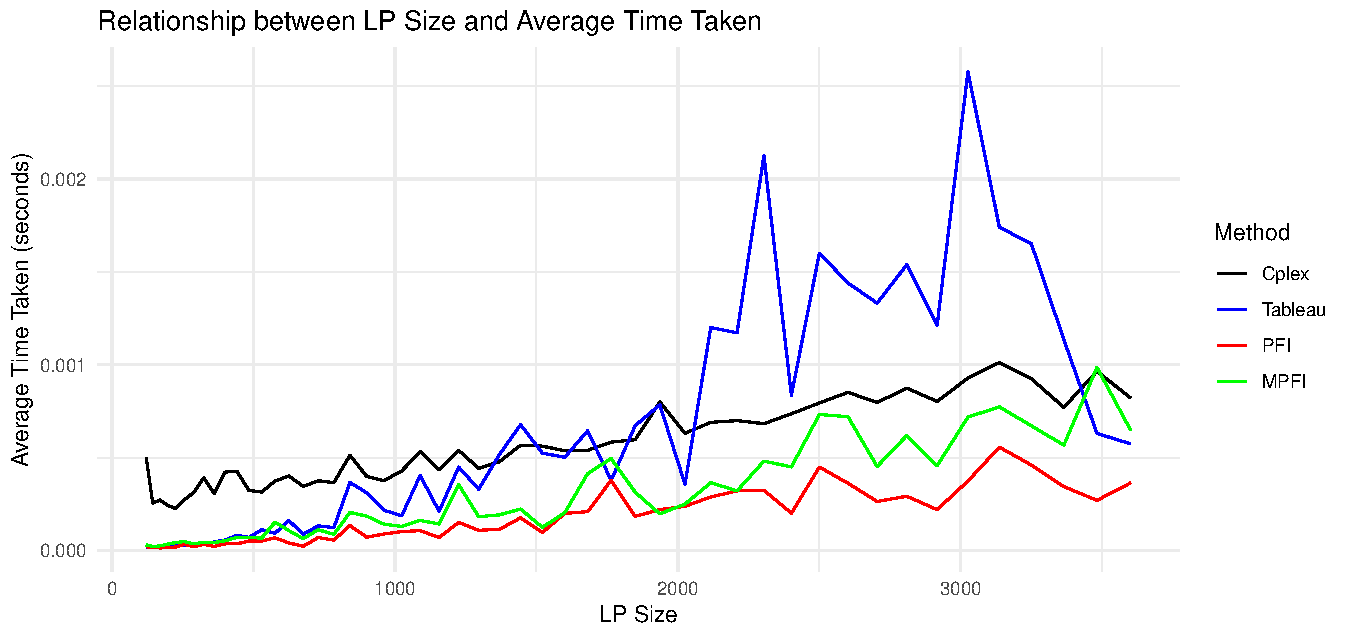
\includegraphics[width=0.8\textwidth]{figures/time_vs_size_random.pdf}
    \caption{Relation between LP size and time for the 3 simplex solvers and Cplex for randomly generated
    dataset with increasing LP size.}
    \label{fig:time_vs_size_random}
\end{figure}


This is our results:
\begin{table}[!htb]
    \centering
    \caption{Number of LPs or Queries Solved by Hour for the randomly generated dataset}
    \begin{tabular}{l|r}
        \toprule
        Method                     & Number of LPs/Queries \\
        \midrule
        Revised Simplex MPFU Umbra & 13,520,349           \\
        Tableau Simplex            & 6,963,530            \\
        Revised Simplex PFI        &  24,352,331          \\
        Cplex                      & 6,666,083             \\
        \bottomrule
    \end{tabular}
\end{table}

We want to see the further evolution of this time profile, so we increase the number of generated LPs 
and explore larger LPs. This provides us with the following results:

\begin{figure}[!htb]
    \centering
    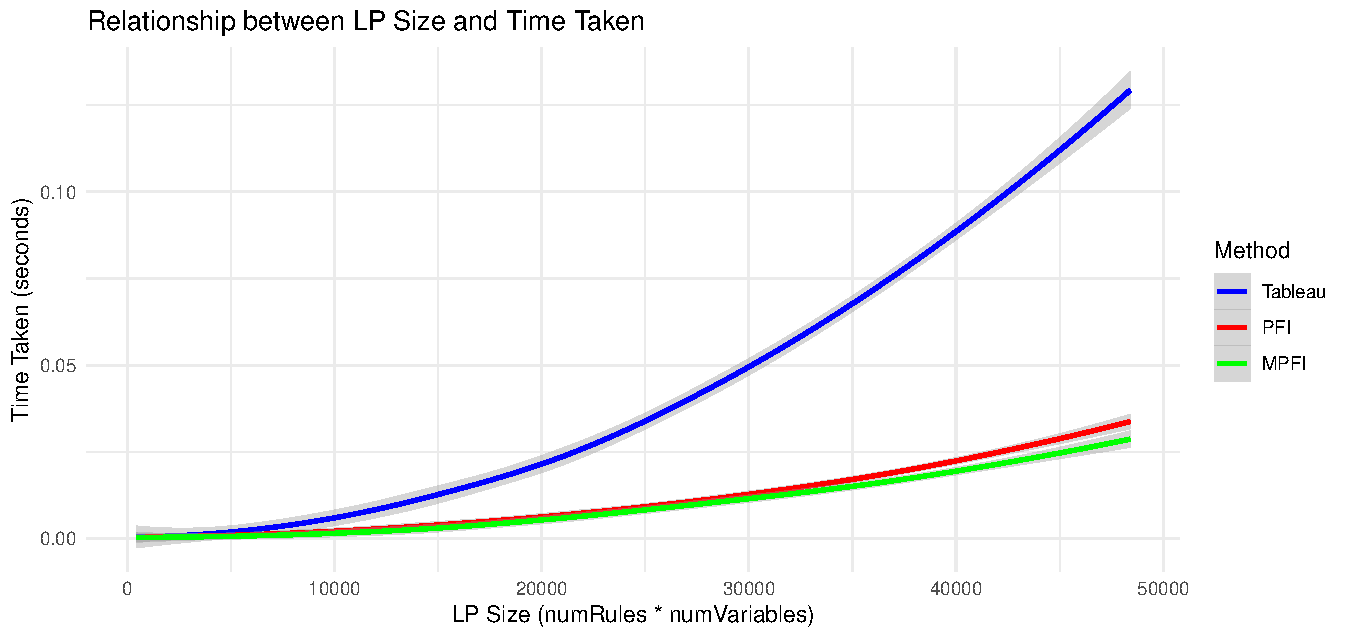
\includegraphics[width=\linewidth]{figures/size_time_random_large.pdf}
    \caption{Relation between LP size and time for the 3 simplex solvers for the randomly generated
    dataset with increasing LP size ranging up to 220 rules and 220 variables.}
    \label{fig:size_time_random_large}
\end{figure}

\begin{figure}[p]
    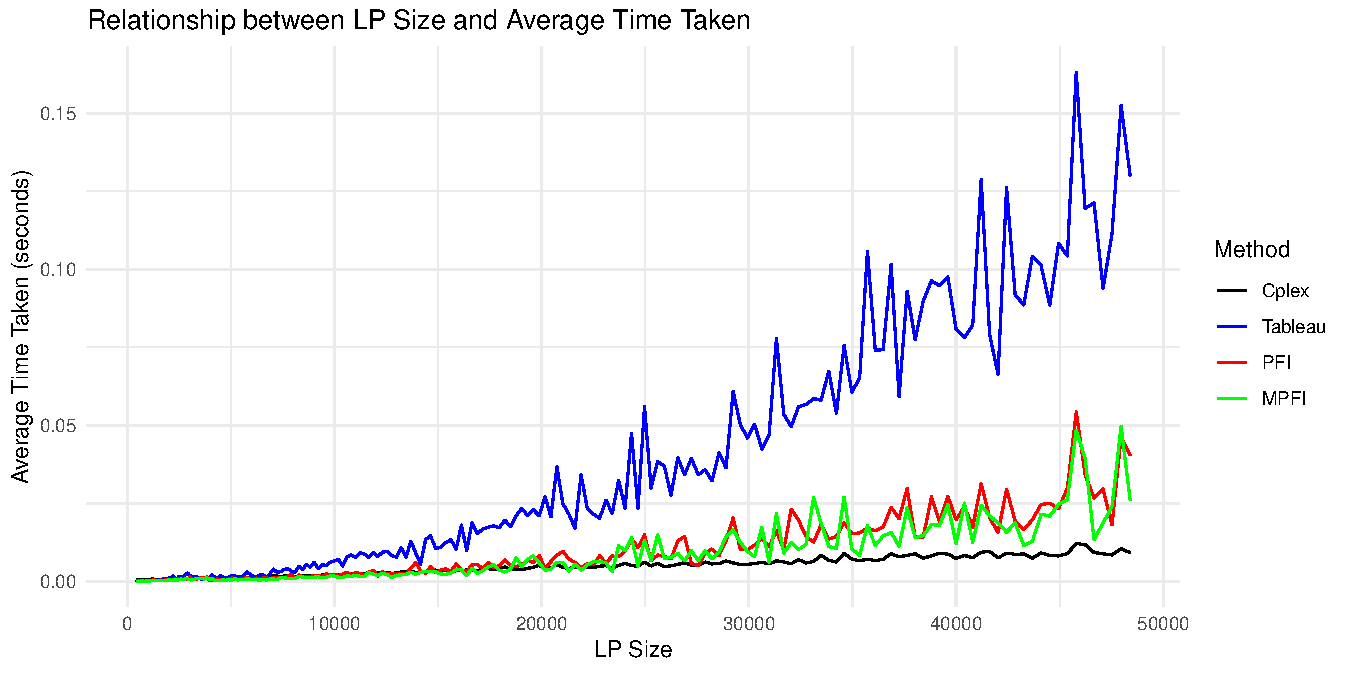
\includegraphics[width=0.8\paperwidth, height=\paperheight, keepaspectratio]{figures/cplex_vs_all_random_large.pdf}
    \caption{Relation between LP size and time for the 3 simplex solvers with CPLEX randomly generated
    dataset with increasing LP size ranging up to 220 rules and 220 variables.}
    \label{cplex_vs_all_random_large}
\end{figure}
%------------------------------------------------------------------------
%------------------------------------------------------------------------
\section{Analysis}

%------------------------------------------------------------------------
\subsection{Dataset Structure}
Our dataset stucture:
as opposed to what the linear programming research has dealt with, which is
very large problems, we are dealing with hundreds of small problems. These are represented
in the revised simplex algorithm by
sparse matrices but not as sparse as it would have been if the problem was large,
small matrices that are not small enough to be dense.
(they still have quite a number of non-zeroes).

%------------------------------------------------------------------------
\subsection{Analysis of dataset properties}
In  this subsection we will conduct an analysis of our dataset properties. What are the
particularites of the structure of these LP problems, is their any patterns in their solution
process. This anaylsis is based on observing the statistical results we obtained from
running different solvers on these problems. This will later provide us with insight
regarding optimization of these problems.
\subsection{Why is highs so slow?}
using \texttt{linprog} from SciPy with HiGHS as a method can be slower than using the HiGHS interface directly, and there are a few reasons for this:

\begin{enumerate}
    \item \textbf{Overhead from Python and SciPy}: When you use \texttt{linprog} from SciPy,
          there's an overhead associated with Python's interpretation and SciPy's function calls.
          This overhead might not be significant for small problems, but for larger LPs or when solving multiple LPs, it can add up.

    \item \textbf{Data Conversion}: \texttt{linprog} has to convert the problem data
          into a format that HiGHS can understand. This conversion can introduce additional computational overhead.

    \item \textbf{Additional Features}: \texttt{linprog} provides a unified interface for
          multiple solvers, and it might perform some additional checks or operations that are not strictly necessary
          when you know you're going to use HiGHS.

    \item \textbf{Version Differences}: Depending on how you installed SciPy and HiGHS,
          there might be version differences between the HiGHS in SciPy and the standalone HiGHS.
          Newer versions of solvers often come with performance improvements, so if SciPy's version is older, it might be slower.

    \item \textbf{Default Parameters}: The default parameters set by \texttt{linprog} for HiGHS
          might not be the most optimal for your specific problem. When using the HiGHS interface directly,
          you have more control over these parameters.
\end{enumerate}

For these reasons, if performance is critical and you're solving large-scale LPs or solving many LPs, it might be beneficial to use
the HiGHS interface directly. However, for many users, the convenience of using
\texttt{linprog} and its unified interface might outweigh the performance benefits of using HiGHS directly.

